%****************************************************************%
%                                                                %
% Modello di tesi di laurea o di dottorato di Lorenzo Pantieri © %
%                                                                %
%         versione: 28 agosto 2012                               %
%                                                                %
%****************************************************************%

% I seguenti commenti speciali impostano:
% 1. utf8 come codifica di input
% 2. PDFLaTeX come motore di composizione
% 3. tesi.tex come documento principale
% 4. il controllo ortografico italiano per l'editor.

% !TEX encoding = UTF-8 Unicode
% !TEX TS-program = pdflatex
% !TEX root = arsclassica.tex
% !TEX spellcheck = it-IT

\documentclass[
              11pt,%                        % primary font size
              a4paper,%                     % A4
%             twoside,openright,%           % double sided
              oneside,openany,%             % only front
              titlepage,%                   % new page after the title
              %fleqn,%                      % position equations at a fixed indent from the left margin rather than centered in the text column (amsmath option)
              headinclude,,footinclude,%    % little header at foot of the page
              BCOR5mm,%                     % 5 mm bookbinding
              numbers=noenddot,%            % niente punto dopo il numero delle sezioni
              cleardoublepage=empty,%       % pagine vuote senza testatina e piede di pagina
              tablecaptionabove,%           % didascalie in cima alle tabelle
              %draft%                       % sostituire con final quando completato
              ]{scrreprt}                   % classe report di KOMA-Script;

\usepackage[T1]{fontenc}                    % codifica dei font:
                                            % NOTA BENE: richiede una distribuzione *completa* di LaTeX (per esempio TeXLive o MiKTeX *complete*)

\usepackage{textcomp}                       % fix warning with missing font shapes
\usepackage{scrhack}                        % fix warnings when using KOMA with listings package
\usepackage{xspace}                         % to get the spacing after macros right

\usepackage[utf8]{inputenc}                 % codifica di input; anche [latin1] va bene
                                            % NOTA BENE! va accordata con le preferenze dell'editor

\usepackage[english]{babel}                 % per scrivere in italiano e in inglese;
                                            % l'ultima lingua (l'italiano) risulta predefinita

\usepackage[suftesi]{frontespizio}          % frontespizo
                                            % per includerlo nel documento bisogna:
                                            % 1. compilare una prima volta tesi.tex;
                                            % 2. compilare a parte tesi-frn.tex, generato dalla compilazione precedente;
                                            % 3. compilare ancora tesi.tex che cercherà il file tesi-frn.pdf

\usepackage{indentfirst}                    % rientra il primo capoverso di ogni sezione

\usepackage{graphicx}                       % immagini

\usepackage{listings}                       % codici

\usepackage[font=small]{quoting}            % citazioni

\usepackage{amsmath,amssymb,amsthm,amsfonts}% matematica

\usepackage[italian]{varioref}              % riferimenti completi della pagina

\usepackage{mparhack,fixltx2e,relsize}      % finezze tipografiche

\usepackage[printonlyused,
            smaller,
            withpage]{acronym}              % acronimi

\usepackage{tabularx}                       % tabelle di larghezza prefissata
%\setlength{\extrarowheight}{3pt}           % increase table row height
%\newcommand{\tableheadline}[1]{\multicolumn{1}{c}{\spacedlowsmallcaps{#1}}}
%\newcommand{\myfloatalign}{\centering}     % to be used with each float for alignment
%\usepackage{caption}
%\captionsetup{format=hang,font=small}

\usepackage[babel,
            italian=guillemets]{csquotes}   % rende automatiche alcune scelte stilistiche dipendenti dalla lingua:
                                            % quando viene usato il comando \mkbibquote si otterranno le virgolette orizzontali invece che quelle verticali
\usepackage[style=philosophy-modern,
            hyperref,backref,natbib,
            backend=biber]{biblatex}       % eccellente pacchetto per la bibliografia;
                                            % philosophy-modern produce uno stile di citazione autore/anno
                                            % aggiungere opzione square dopo backref per parentesti quadrate invece che tonde
                                            % numeric-comp produce riferimenti numerici

\bibliography{bibliography}                 % database di biblatex

\usepackage{subfig}                         % sottofigure, sottotabelle

\usepackage{lipsum}                         % testo fittizio

\usepackage{eurosym}                        % simbolo dell'euro

% ********************************************************************
% Available options for classicthesis.sty:
% drafting
% parts nochapters linedheaders
% eulerchapternumbers beramono eulermath pdfspacing minionprospacing
% tocaligned dottedtoc manychapters
% listings floatperchapter subfig
% ********************************************************************
\usepackage[eulerchapternumbers,%           % numeri dei capitoli nel font Euler
            subfig,%                        % se si usa il pacchetto subfig
            %minionpro,                     %
            beramono,%                      % Bera Mono come font a spaziatura fissa
            eulermath,%                     % AMS Euler come font per la matematica
            pdfspacing,%                    % migliora il riempimento di riga
            listings,%                      % codici
            %parts,%                        % da decommentare in un documento diviso in parti
            dottedtoc,%                     % allinea a destra i numeri di pagina nell'indice
            floatperchapter                 % numerazione per capitolo dei float (e.g. tabelle, figure, listings)
            ]{classicthesis}                % stile classicthesis


\usepackage{arsclassica}                    % modifica alcuni aspetti di classicthesis

\usepackage{bookmark}                       % segnalibri

\usepackage{etoolbox}

\usepackage[noabbrev]{cleveref}

\usepackage{chngcntr}

\usepackage{makeidx}                        % indice analitico

\usepackage{multicol}

%******************************************************************
% Settings
%******************************************************************
% settings.tex
%*********************************************************************************

%*********************************************************************************
% Comandi personali
%*********************************************************************************
\newcommand{\myName}{Leonardo~Di~Donato}% author
\newcommand{\myTitle}{Continuos Time Bayesian Networks Classifiers}% title
\newcommand{\myDegree}{Tesi di Laurea}% tipo di tesi
\newcommand{\myUni}{Universit� degli Studi di Milano--Bicocca}% university
\newcommand{\myFaculty}{Facolt� di Scienze Matematiche, Fisiche e Naturali}% facolt�
\newcommand{\myDepartment}{Dipartimento di Informatica, Sistemistica e Comunicazione}% dipartimento
\newcommand{\myProf}{Prof.~F.~Antonio~Stella}% relatore
\newcommand{\myOtherProf}{Dott.~Daniele~Codecasa}% correlatore
\newcommand{\myLocation}{Milano}% dove
\newcommand{\myTime}{Settembre 2013}% quando
\newcommand{\mySubject}{Continuos time Bayesian Networks}
\newcommand{\myKeywords}{Classification, Continuos time Bayesian Network, CTBN, Continuos time Bayesian Newtork Classifier, CTBNC}

%*********************************************************************************
% TOC settings
%*********************************************************************************
% \setcounter{secnumdepth}{5}
% \setcounter{tocdepth}{5}

%*********************************************************************************
% Chapters style
%*********************************************************************************
% Chapter number style: decomment if you want it with the same corpus font
% \renewcommand{\chapterNumber}{%
% \fontsize{70}{70}\usefont{\encodingdefault}{\sfdefault}{b}{n}%
% }%

% Workaround: multi-line titles
\renewcommand\formatchapter[1]{%
\begin{minipage}[b]{0.15\linewidth}
\chapterNumber
\end{minipage}%
\begin{minipage}[b]{0.70\linewidth}%length of the second row
\raggedright\spacedallcaps{#1}
\end{minipage}
}

%*********************************************************************************
% Analytical index
%*********************************************************************************
\makeindex

% Balance columns of the last page
% \let\orgtheindex\theindex
% \let\orgendtheindex\endtheindex
% \def\theindex{%
% \def\twocolumn{\begin{multicols}{2}}%
% \def\onecolumn{}%
% \clearpage
% \orgtheindex
% }
% \def\endtheindex{%
% \end{multicols}%
% \orgendtheindex
% }

% Indexing commands
\newcommand*{\keyword}[2][]{#2\index{#2@#2#1}}% as simple keyword
\newcommand{\keywordsub}[2][]{#2\index{#1!#2}}% as categorized keyword
\newcommand{\keywordpagb}[1]{\keyword[|textbf]{#1}}% as simple keyword with bold page number
\newcommand{\keywordpagi}[1]{\keyword[|textit]{#1}}% as simple keyword with italic page number
\newcommand{\keywordbold}[1]{#1\index{#1@\textbf{#1}}}% as bold keyword
\newcommand{\keyworditalic}[1]{#1\index{#1@\textsl{#1}}}% as italic keyword

%*********************************************************************************
% Impostazioni di amsmath, amssymb, amsthm
%*********************************************************************************
% force the equation numbers to be always the same size
\makeatletter
\renewcommand{\maketag@@@}[1]{\hbox{\m@th\normalsize\normalfont#1}}%
\makeatother

% operators
\DeclareMathOperator*{\argmax}{arg\,max}
\DeclareMathOperator*{\argmin}{arg\,min}

% comandi per gli insiemi numerici (serve il pacchetto amssymb)
\newcommand{\numberset}{\mathbb}
\newcommand{\N}{\numberset{N}}
\newcommand{\R}{\numberset{R}}

% comandi per gli insiemi
\newcommand{\set}[1]{\mathbf{#1}}
\newcommand{\setel}[1]{\mathnormal{#1}}  % o \mathrm o \mathit

% comandi per i vettori
\newcommand{\vect}[1]{\set{#1}}
\newcommand{\vectel}[1]{\mathrm{#1}}

% comandi per i simboli matematici che denotano schemi, categorie, concetti
\newcommand{\conceptsym}[1]{\mathcal{#1}}

% un ambiente per i sistemi
\newenvironment{sistema}%
  {\left\lbrace\begin{array}{@{}l@{}}}%
  {\end{array}\right.}

% comandi per le lettere greche
% ...

% reference for equation terms. use \underbrace{equation}_{\myterm{termA}}
\newcounter{term}
\renewcommand*{\theterm}{(\alph{term})}
\AtBeginDocument{%
  \let\mylabel\label
}
\newcommand{\myterm}[1]{%
  \begingroup % keep the effects of \refstepcounter local
    \refstepcounter{term}%
    \mylabel{#1}%
    \text{\theterm}%
  \endgroup
}

%*********************************************************************************
% Nuovi ambienti: definizioni, teoremi etc. etc.
%*********************************************************************************
% definizioni (serve il pacchetto amsthm)
\newtheoremstyle{classicdef}% Nome
{12pt}% Spazio che precede l�enunciato
{12pt}% Spazio che segue l�enunciato
{}% Stile del font dell�enunciato
{}% Rientro (se vuoto, non c�� rientro,
% \parindent = rientro dei capoversi)
{\scshape}% Stile del font dell�intestazione
{:}% Punteggiatura che segue l�intestazione
{.5em}% Spazio che segue l�intestazione:
% " " = normale spazio inter-parola;
% \newline = a capo
{}% Specifica l�intestazione dell�enunciato
% (normalmente viene lasciata vuota)

\theoremstyle{definition}
\newtheorem{definizione}{Definizione}
% \newtheorem{osservazione}[definizione]{Osservazione}
% \newtheorem{definizione}{Definizione}[section]
\newtheorem{osservazione}{Osservazione}[definizione]

% esempi
\theoremstyle{definition}
\newtheorem{esempio}{Esempio}[definizione]

% note about definitions
\theoremstyle{remark}
\newtheorem{notabene}{Nota}[definizione]

% note of section
\theoremstyle{remark}
\newtheorem{nota}{Nota}[section]

% teoremi (serve il pacchetto amsthm)
\newtheoremstyle{classicthm}% Nome
{12pt}% Spazio che precede l�enunciato
{12pt}% Spazio che segue l�enunciato
{\itshape}% Stile del font dell�enunciato
{}% Rientro (se vuoto, non c�� rientro,
% \parindent = rientro dei capoversi)
{\scshape}% Stile del font dell�intestazione
{:}% Punteggiatura che segue l�intestazione
{.5em}% Spazio che segue l�intestazione:
% " " = normale spazio inter-parola;
% \newline = a capo
{}% Specifica l�intestazione dell�enunciato
% (normalmente viene lasciata vuota)

\theoremstyle{plain}
\newtheorem{teorema}{Teorema}[chapter]
\newtheorem*{teorema*}{Teorema}
\newtheorem{cor}[teorema]{Corollario}
\newtheorem{lem}[teorema]{Lemma}
\newtheorem{prop}[teorema]{Proposizione}
\newtheorem{oss}[teorema]{Osservazione}

% leggi (serve il pacchetto amsthm)
\newtheorem{legge}{Legge}
\newtheorem{decreto}[legge]{Decreto}

%*********************************************************************************
% Impostazioni di acronym
%*********************************************************************************
\newcommand{\acroname}{Acronimi}
% \renewcommand*{\acsfont}[1]{\textssc{#1}}                 % for MinionPro
\renewcommand*{\acsfont}[1]{\textsmaller{#1}}               % customize font for long version acronyms [works only if footnote not activate]
\renewcommand*{\acffont}[1]{#1}                             % idem, but for short version of acronyms
\renewcommand{\bflabel}[1]{{#1}\hfill}                      % fix the list of acronyms
\makeatletter                                               % macro that tweeks acronym package to rendere lowercase or not
\newif\if@in@acrolist
\AtBeginEnvironment{acronym}{\@in@acrolisttrue}
\newrobustcmd{\ul}[2]{\if@in@acrolist#1\else#2\fi}          % \ul{C}{c}iao defines an uppercase and lowercase variant of the same acronym
\newcommand{\ACF}[1]{{\@in@acrolisttrue\acf{#1}}}           % \ACF{<acronym>} force the defined capitalized variants of acronym letters/words
\newcommand{\ACL}[1]{{\@in@acrolisttrue\acl{#1}}}           % \ACL{<acronym}
\makeatother

%*********************************************************************************
% Impostazioni di biblatex
%*********************************************************************************
\defbibheading{bibliography}{%
\cleardoublepage
\manualmark
\phantomsection
\addcontentsline{toc}{chapter}{\tocEntry{\bibname}}
\chapter*{\bibname\markboth{\spacedlowsmallcaps{\bibname}}
{\spacedlowsmallcaps{\bibname}}}}

%*********************************************************************************
% Definizione di un linguaggio di pseudo-codice
%*********************************************************************************
\lstdefinelanguage{pseudo}{
    morekeywords=%
    {
        for,foreach,return,if,else,ifelse,max,min,in,len,log,index,var,function,seqlen,as,new,while,unique,which
    },
    morecomment=[l][\color{Green}\ttfamily]{//},
    morecomment=[s][\color{Green}\ttfamily]{/*}{*/},
    morestring=[b][\color{Red}\rmfamily]",
    moredelim=[is][\color{Orange}]{|*}{*|}
}

%*********************************************************************************
% Impostazioni di listings
%*********************************************************************************
\lstset{
    %language=pseudo,%[LaTeX]Tex,%C++,
    basicstyle=\normalsize\ttfamily,
    % identifierstyle=\color{NavyBlue},
    % keywordstyle=\bfseries,%\color{RoyalBlue},%\bfseries,
    % commentstyle=\color{Green}\ttfamily,
    % stringstyle=\rmfamily,
    numbers=left,%none
    numberstyle=\scriptsize,%\tiny
    stepnumber=1,
    numbersep=8pt,
    showstringspaces=false,
    breaklines=true,
    frameround=ftff,%fttt,%
    frame=TB,%lines,
    tabsize=1,
    escapeinside={<ls>}{<le>}
}

% Dichiarazioni utili per l'indice della tesi e le etichette
\addto\captionsitalian{%
\renewcommand{\lstlistingname}{Algoritmo}}
\addto\captionsitalian{%
\renewcommand{\lstlistlistingname}{Elenco degli algoritmi}}
\providecommand*{\lstlistingautorefname}{algoritmo}
\providecommand*{\lstnumberautorefname}{linea}

%*********************************************************************************
% Impostazioni di hyperref
%*********************************************************************************
\hypersetup{%
    % hyperfootnotes=false,pdfpagelabels,
    %draft,	% = elimina tutti i link (utile per stampe in bianco e nero)
    colorlinks=true, linktocpage=true, pdfstartpage=1, pdfstartview=FitV,%
    % decommenta la riga seguente per avere link in nero (per esempio per la stampa in bianco e nero)
    % colorlinks=false, linktocpage=false, pdfborder={0 0 0}, pdfstartpage=1, pdfstartview=FitV,%
    breaklinks=true, pdfpagemode=UseNone, pageanchor=true, pdfpagemode=UseOutlines,%
    plainpages=false, bookmarksnumbered, bookmarksopen=true, bookmarksopenlevel=1,%
    hypertexnames=true, pdfhighlight=/O,%nesting=true,%frenchlinks,%
    urlcolor=webbrown, linkcolor=RoyalBlue, citecolor=webgreen, %pagecolor=RoyalBlue,%
    urlcolor=Black, linkcolor=Black, citecolor=Black, %pagecolor=Black,%
    pdftitle={\myTitle},%
    pdfauthor={\textcopyright\ \myName, \myUni, \myFaculty},%
    pdfsubject={\mySubject},%
    pdfkeywords={\myKeywords},%
    pdfcreator={pdfLaTeX},%
    pdfproducer={LaTeX with hyperref, classicthesis and arsclassica}%
}

%*********************************************************************************
% Impostazioni di graphicx
%*********************************************************************************
\graphicspath{{images/}} % cartella dove sono riposte le immagini

%*********************************************************************************
% Margini ottimizzati per l'A4
%*********************************************************************************
\areaset[current]{336pt}{750pt}
\setlength{\marginparwidth}{7em}
\setlength{\marginparsep}{2em}%

%*********************************************************************************
% Utility
%*********************************************************************************
% make first letter uppercase
\makeatletter
\def\upcase{\expandafter\makeupcase}
\def\makeupcase#1{\uppercase{#1}}
\makeatother

% make first letter lowercase
\makeatletter
\def\lwcase{\expandafter\makelwcase}
\def\makelwcase#1{\lowercase{#1}}
\makeatother

%*********************************************************************************
% References
%*********************************************************************************
\addto\extrasitalian{%
  \def\equationautorefname{equazione}%
}
\addto\extrasitalian{%
  \def\chapterautorefname{capitolo}%
}
\addto\extrasitalian{%
  \def\sectionautorefname{sezione}%
}
\addto\extrasitalian{%
  \def\subsectionautorefname{sottosezione}%
}
\addto\extrasitalian{%
  \def\subsubsectionautorefname{sottosezione}%
}

%*********************************************************************************
% Custom references for \autoref
%*********************************************************************************
\newcommand{\definizioneautorefname}{definizione}
\newcommand{\osservazioneautorefname}{osservazione}
\newcommand{\notabeneautorefname}{nota}
\newcommand{\esempioautorefname}{esempio}
\newcommand{\termautorefname}{termine}
\newcommand{\teoremaautorefname}{teorema}

%*********************************************************************************
% Set footnote's continuos numbering and linking capabilities (using cleveref and chngcntr packages)
%*********************************************************************************
\counterwithout{footnote}{chapter}
\crefformat{footnote}{#2\footnotemark[#1]#3}

%*********************************************************************************
% Altro
%*********************************************************************************
% ...
\newcommand{\omissis}{\dots\negthinspace}
\newcommand{\virgolette}[1]{``#1''}
\newcommand{\caporali}[1]{�#1�}

%
\newcommand{\ie}{i.\,e.}
\newcommand{\Ie}{I.\,e.}
\newcommand{\eg}{e.\,g.}
\newcommand{\Eg}{E.\,g.}

% comuni
\newcommand{\ct}{continuos time}
\newcommand{\nb}{Na\"ive Bayes}
\newcommand{\bn}{Bayesian Network}
\newcommand{\class}{classifier}
\newcommand{\ctbn}{\upcase \ct{} \bn{}}
\newcommand{\ctnb}{\upcase \ct{} \nb{}}
\newcommand{\cttanb}{\upcase \ct{} tree augumented \nb{}}
\newcommand{\stats}{statistiche sufficienti}
\newcommand{\pv}{variabile di processo}

\makeatletter
\newcommand{\omog}{omogene\@ifstar{o}{i}}
\makeatother

\makeatletter
\newcommand{\cond}{condizional\@ifstar{e}{i}}
\makeatother

\makeatletter
\newcommand{\im}{matric\@ifstar{e di intensit\`a}{i di intensit\`a}}
\makeatother

\makeatletter
\newcommand{\cim}{\@ifstar{\im*{} \cond*}{\im{} \cond}}
\makeatother

\makeatletter
\newcommand{\mprocess}{process\@ifstar{o di Markov}{i di Markov}}
\makeatother

\makeatletter
\newcommand{\ctmp}{\@ifstar{\mprocess*{} a tempo continuo}{\mprocess{} a tempo continuo}}
\makeatother

% elementi matematici comuni
\newcommand{\imsign}[1]{\set{Q}_{#1}}
\newcommand{\cimsign}[2]{\imsign{\,#1\,\arrowvert\,#2}}
\newcommand{\priorsign}[1]{\set{P}^0_{#1}}
\newcommand{\tstat}[1]{T[\,\setel{#1}\,]}
\newcommand{\mstat}[2][]{
    \ifstrempty{#1}{%
        M[\,\setel{#2}\,]%
    }{%
        M[\,\setel{#1}\,,\,#2\,]%
    }%
}
\newcommand{\param}[1]{\boldsymbol{\textbf{\text{#1}}}}
\newcommand{\paramhat}[1]{\boldsymbol{\hat{\textbf{#1}}}}
\newcommand{\greekhat}[1]{\boldsymbol{\skew{-.5}\hat#1}}
\newcommand{\evidencestream}[1]{(\set{x}^1\,,\,\set{x}^2\,,\,\dotsc\,,\,\set{x}^{#1})}

%*********************************************************************************
% Eccezioni all'algoritmo di sillabazione
%*********************************************************************************
\hyphenation{Fortran ma-cro-istru-zio-ne nitro-idrossil-amminico tem-po-ra-li}


                            % file con le impostazioni personali
%******************************************************************
% Document
%******************************************************************
\begin{document}
\pagestyle{scrheadings}
\pagenumbering{roman}
%******************************************************************
% Front matter
%******************************************************************
% !TEX encoding = UTF-8
% !TEX TS-program = pdflatex
% !TEX root = ../arsclassica.tex
% !TEX spellcheck = it-IT

%*******************************************************
% Frontispiece
%*******************************************************
\begin{frontespizio}
\Preambolo{\usepackage{iwona}} % riga da commentare se non si carica arsclassica

\Universita{Place}
\Logo{images/sigillo}
\Facolta{Mathematics}
\Corso{Computer Science}
\Annoaccademico{2012--2013}
\Titoletto{M.Sc Degree}
\Titolo{Thesis title}
\Sottotitolo{Thesis subtitle}
\Candidato[744739]{Name~Surname}
\Relatore{Prof.~F.~Second~Surname}
\Correlatore{Dott.~Name~Surname}
\end{frontespizio}

% !TEX encoding = UTF-8
% !TEX TS-program = pdflatex
% !TEX root = ../arsclassica.tex
% !TEX spellcheck = it-IT

%*******************************************************
% Colophon
%*******************************************************
\clearpage
\phantomsection
\thispagestyle{empty}

\hfill

\vfill

\noindent\myname: \textit{\mytitle}
\mydegree \hspace{1px} \textcopyright\ \MakeTextLowercase{\mytime}.

\lipsum[2]

% !TEX encoding = UTF-8
% !TEX TS-program = pdflatex
% !TEX root = ../arsclassica.tex
% !TEX spellcheck = it-IT

%*******************************************************
% Dedication
%*******************************************************
\cleardoublepage
\phantomsection
\thispagestyle{empty}
\pdfbookmark{Dedication}{Dedication}

\vspace*{3cm}

\begin{center}
Lorem ipsum dolor sit amet, consectetuer adipiscing elit. \\ \medskip
--- Donald Knuth    
\end{center}

\medskip

\begin{center}
Dedicated to all the lovers of \LaTeX.
\end{center}

% !TEX encoding = UTF-8
% !TEX TS-program = pdflatex
% !TEX root = ../arsclassica.tex
% !TEX spellcheck = it-IT

%*******************************************************
% Indexes
%*******************************************************
\cleardoublepage
\pdfbookmark{\contentsname}{tableofcontents}
\tableofcontents
\markboth{\spacedlowsmallcaps{\contentsname}}{\spacedlowsmallcaps{\contentsname}}
\clearpage

\begingroup
    \let\clearpage\relax
    \let\cleardoublepage\relax
    \let\cleardoublepage\relax

    %*******************************************************
    % List of figures
    %*******************************************************
    \phantomsection
    \pdfbookmark{\listfigurename}{lof}
    \listoffigures

    \vspace*{8ex}

    %*******************************************************
    % List of tables
    %*******************************************************
    \phantomsection
    \pdfbookmark{\listtablename}{lot}
    \listoftables

    \vspace*{8ex}

    %*******************************************************
    % List of listings
    %*******************************************************
    \phantomsection
    \pdfbookmark{\lstlistlistingname}{loa}
    \lstlistoflistings

    \vspace*{8ex}

\endgroup

\cleardoublepage

% !TEX encoding = UTF-8
% !TEX TS-program = pdflatex
% !TEX root = ../arsclassica.tex
% !TEX spellcheck = it-IT

%*******************************************************
% Summary and Abstract
%*******************************************************
\cleardoublepage
\phantomsection
\pdfbookmark{Summary}{Summary}
\begingroup
\let\clearpage\relax
\let\cleardoublepage\relax
\let\cleardoublepage\relax

\chapter*{Summary}

\lipsum[1]

\vfill

\pdfbookmark{Abstract}{Abstract}
\chapter*{Abstract}

\lipsum[2]

\endgroup			

\vfill


% !TEX encoding = UTF-8
% !TEX TS-program = pdflatex
% !TEX root = ../arsclassica.tex
% !TEX spellcheck = it-IT

%*******************************************************
% Acknowledgements
%*******************************************************
\cleardoublepage
\phantomsection
\pdfbookmark{Acknowledgements}{Acknowledgements}

\begin{flushright}{\slshape    
	Lorem ipsum dolor sit amet, consectetuer adipiscing elit. \\
	Ut purus elit, vestibulum ut, placerat ac, adipiscing vitae, felis. \\
	Curabitur dictum gravida mauris.} \\ \medskip
    --- Donald Ervin Knuth
\end{flushright}


\bigskip

\begingroup
\let\clearpage\relax
\let\cleardoublepage\relax
\let\cleardoublepage\relax

\chapter*{Acknowledgements}

\lipsum[1]

\bigskip
 
\noindent\textit{\myLocation, \MakeTextLowercase{\myTime}}
\hfill ~L.

\endgroup

% !TEX encoding = UTF-8
% !TEX TS-program = pdflatex
% !TEX root = ../arsclassica.tex
% !TEX spellcheck = it-IT

%*******************************************************
% Introduction
%*******************************************************
\cleardoublepage
\pdfbookmark{Introduction}{Introduction}
\chapter*{Introduction}\label{cap:intro}

\lipsum[1]

Lorem ipsum dolor sit amet, consectetuer adipiscing elit.
% \begin{description}
% \item[{\hyperref[cap:lorem]{Il primo capitolo}}]
% offre una visione d'insieme della storia di \LaTeX{} e ne vengono presentate le idee di fondo.
% \item[{\hyperref[cap:ipsum]{Il secondo capitolo}}]
% spiega le operazioni, veramente semplici, per installare \LaTeX{} sul proprio calcolatore.
% \item[{\hyperref[cap:dolor]{L'appendice A}}] descrive  sinteticamente le principali norme tipografiche della lingua italiana, utili nella composizione di articoli, tesi o libri.
% \end{description}

\begin{description}
\item[{\hyperref[cap:one]{First chapter}}]
talks about \omissis{}
\item[{\hyperref[cap:two]{Second chapter}}]
talks about \omissis{}
\item[{\hyperref[cap:three]{Third chapter}}]
talks about \omissis{}
\end{description}

% \lipsum[2]

\cleardoublepage
%******************************************************************
% Body matter
%******************************************************************
\pagenumbering{arabic}
% !TEX encoding = UTF-8
% !TEX TS-program = pdflatex
% !TEX root = ../arsclassica.tex
% !TEX spellcheck = it-IT

%************************************************
\chapter{One}
\label{cap:one}
%************************************************

A citation~\citep{gihman1973}. And another citation~\citep{gihman1974}

Lorem \keyword{ipsum} \keyword{dolor} sit \keyword{amet}, consectetuer adipiscing elit. Ut purus elit, vestibulum ut, placerat ac, adipiscing vitae, felis. Curabitur dictum gravida mauris. Nam arcu libero, nonummy eget, consectetuer id, vulputate a, magna. Donec vehicula augue eu neque.

\section{Examples}

\subsection{Tables}

\lipsum

\begin{table}[tb]
\caption[A floating table]{And example showing a floating table.}
\label{tab:ex-1}
\centering
\begin{tabular}{cc}
\toprule
$p$ & $\lnot p$ \\ 
\midrule
V   & F \\ 
F   & V \\
\bottomrule 
\end{tabular}
\end{table}

The ~\vref{tab:ex-1} provides an example of floating table.

\lipsum[1-2]

\subsection{Figure}

\lipsum[2]

\begin{figure}[tb] 
\centering 
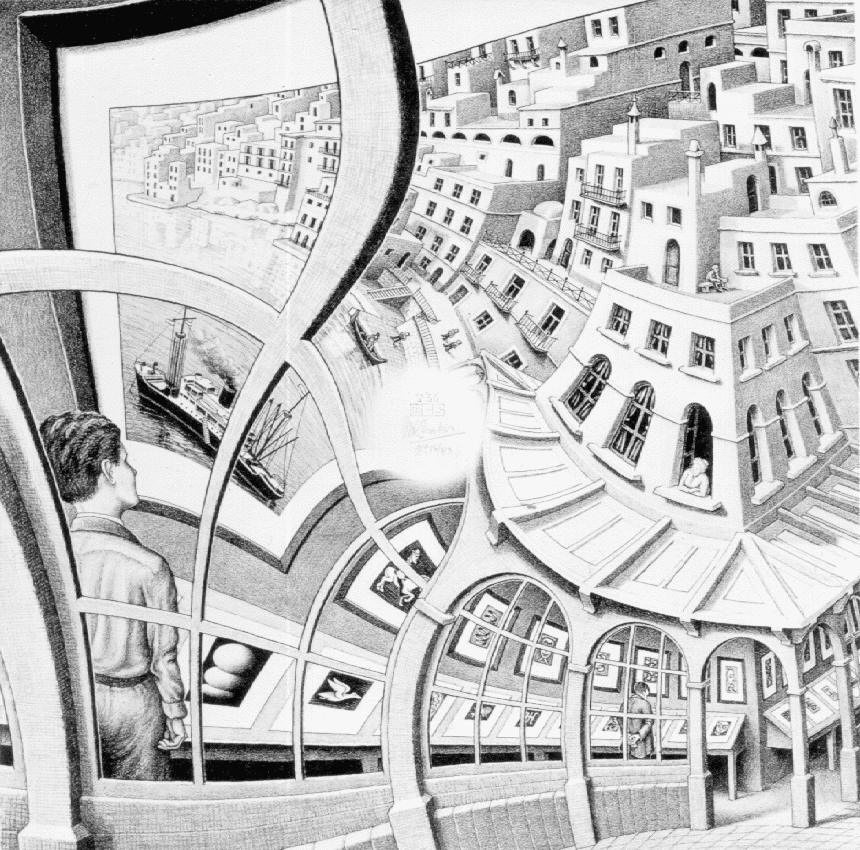
\includegraphics[width=0.5\columnwidth]{gallery} 
\caption[Un esempio di figura mobile]{Un esempio di figura mobile (l'immagine, che riproduce la litografia \emph{Galleria di stampe}, di M.~Escher,\index{Escher, M.~C.} proviene da \url{http://www.mcescher.com/}).}
\label{fig:galleria} 
\end{figure}

La figura~\vref{fig:galleria} fornisce un esempio di figura mobile.

\lipsum[3]

\begin{figure}[tb]
\centering
\subfloat[Asia personas duo.]
{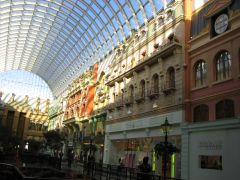
\includegraphics[width=.45\columnwidth]{lorem}} \quad
\subfloat[Pan ma signo.]
{\label{fig:ipsum}%
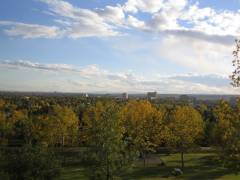
\includegraphics[width=.45\columnwidth]{ipsum}} \\
\subfloat[Methodicamente o uno.]
{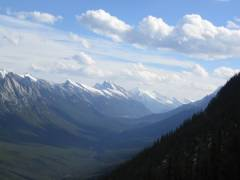
\includegraphics[width=.45\columnwidth]{dolor}} \quad
\subfloat[Titulo debitas.]
{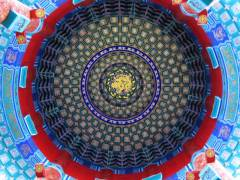
\includegraphics[width=.45\columnwidth]{sit}}
\caption[Tu duo titulo debitas latente]{Tu duo titulo debitas
latente.}
\label{fig:esempio}
\end{figure}

La figura~\vref{fig:esempio} costituisce un esempio di figura mobile.

\lipsum[4]

% !TEX encoding = UTF-8
% !TEX TS-program = pdflatex
% !TEX root = ../arsclassica.tex
% !TEX spellcheck = it-IT

%************************************************
\chapter{Ipsum}
\label{cap:ipsum}
%************************************************


Lorem ipsum dolor sit amet, consectetuer adipiscing elit. Nam dui ligula, fringilla a, euismod sodales, sollicitudin vel, wisi. Morbi auctor lorem non justo. Nam lacus libero, pretium at, lobortis vitae, ultricies et, tellus.
\begin{description}
\item[Lorem ipsum dolor] sit amet, consectetuer adipiscing elit. Ut purus elit, vestibulum ut, placerat ac $\lim_{n \to \infty}\sum_{k=1}^n \frac{1}{k^2}= \frac{\pi^2}{6}$.
\item[Mauris ut leo.]
Cras viverra metus rhoncus sem. Nulla et lectus vestibulum urna fringilla ultrices. Phasellus eu tellus sit amet tortor gravida placerat.
\[
\lim_{n \to \infty}\sum_{k=1}^n \frac{1}{k^2}= \frac{\pi^2}{6}.
\]
\end{description}

Nulla malesuada porttitor diam. Donec felis erat, congue non, volutpat at, tincidunt tristique, libero. Vivamus viverra fermentum felis.
\begin{equation}
\label{eq:euler}
e^{i\pi}+1=0.
\end{equation}
Dalla formula~\eqref{eq:euler} 
si deduce che\dots






\section{Nozioni basilari}

\subsection{Insiemi numerici}

Donec nonummy pellentesque ante. Phasellus adipiscing semper elit.
\begin{equation}
x^2 \geq 0 \quad
\forall x \in \mathbb{R}.
\end{equation}


\subsection{Le matrici}

\lipsum[2]
\begin{equation}
A=
\begin{bmatrix}
x_{11} & x_{12} & \dots \\
x_{21} & x_{22} & \dots \\
\vdots & \vdots & \ddots
\end{bmatrix}
\end{equation}



\section{Formule fuori corpo}

Proin fermentum massa ac quam. Sed diam turpis, molestie vitae, placerat a, molestie nec, leo. Maecenas lacinia. Nam ipsum ligula, eleifend at, accumsan nec, suscipit a, ipsum. 


\subsection{Una formula spezzata con allineamento}

\lipsum[2]
\begin{equation} 
\begin{split} 
a &= b+c-d \\ 
  &= e-f \\ 
  &= g+h \\ 
  &= i. 
\end{split} 
\end{equation}

 
\subsection{Casi}

\lipsum[3]
\begin{equation}
f(n):=
\begin{cases} 
2n+1, & \text{con $n$ dispari,} \\ 
n/2,  & \text{con $n$ pari.} 
\end{cases} 
\end{equation}



\section{Enunciati e dimostrazioni}

Nunc eleifend consequat lorem. Sed lacinia nulla vitae enim. Pellentesque tincidunt purus vel magna. Integer non enim. Praesent euismod nunc eu purus.
\begin{definizione}[di Gauss] 
Un \emph{matematico} trova ovvio che
$\int_{-\infty}^{+\infty}
e^{-x^2}\,dx=\sqrt{\pi}$. 
\end{definizione} 
\begin{teorema} 
I matematici, se ce ne sono, sono molto rari.
\end{teorema} 

\lipsum[2]

\begin{teorema}[di Pitagora]
La somma dei quadrati costruiti sui cateti uguaglia il quadrato costruito sull'ipotenusa.
\end{teorema}
La dimostrazione viene lasciata per esercizio.

Donec bibendum quam in tellus. Nullam cursus pulvinar lectus. Donec et mi. Nam vulputate metus eu enim. Vestibulum pellentesque felis eu massa.
\begin{teorema}[Sorpresa]
Si ha che $\log(-1)^2=2\log(-1)$.
\end{teorema} 
\begin{proof} 
Si ha che $\log(1)^2 = 2\log(1)$.
Ma si ha anche che $\log(-1)^2=\log(1)=0$.
Quindi $2\log(-1)=0$, da cui la tesi.
\end{proof}
Viene un quadratino a fine dimostrazione.
\begin{legge}
\label{lex:capo}
Il capo ha ragione.
\end{legge}
\begin{decreto}[Aggiornamento alla legge~\ref{lex:capo}]
Il capo ha \emph{sempre} ragione.
\end{decreto}
\begin{legge}
Se il capo ha torto, vedere la 
legge~\ref{lex:capo}.
\end{legge}


Nam dui ligula, fringilla a, euismod sodales, sollicitudin vel, wisi. Morbi auctor lorem non justo. Nam lacus libero, pretium at, lobortis vitae, ultricies et, tellus.

Cras nec ante. Pellentesque a nulla. Cum sociis natoque penatibus et magnis dis parturient montes, nascetur ridiculus mus. Aliquam tincidunt urna.

% !TEX encoding = UTF-8
% !TEX TS-program = pdflatex
% !TEX root = ../arsclassica.tex
% !TEX spellcheck = it-IT

%************************************************
\chapter{Dolor}
\label{cap:dolor}
%************************************************

\lipsum[1]

\section{Mane}
\lipsum[2]

\section{Tekel}
\lipsum[3]

\section{Fares}
\lipsum[4-5]

% *****************************************************************
% Backmatter
%******************************************************************
\appendix
% !TEX encoding = UTF-8
% !TEX TS-program = pdflatex
% !TEX root = ../arsclassica.tex
% !TEX spellcheck = it-IT

%************************************************
\chapter{Code}
\label{cap:appendix-1}
%************************************************

\lipsum[1]

% !TEX encoding = UTF-8
% !TEX TS-program = pdflatex
% !TEX root = ../arsclassica.tex
% !TEX spellcheck = it-IT

%************************************************
\chapter{Ipsum}
\label{cap:appendix-2}
%************************************************

\lipsum[2]

% !TEX encoding = UTF-8
% !TEX TS-program = pdflatex
% !TEX root = ../arsclassica.tex
% !TEX spellcheck = it-IT

%*******************************************************
% Acronnyms
%*******************************************************
\cleardoublepage
\manualmark
\phantomsection
\addcontentsline{toc}{chapter}{\tocEntry{\acroname}}
\chapter*{\acroname\markboth{\spacedlowsmallcaps{\acroname}}{\spacedlowsmallcaps{\acroname}}}
\small
\begin{acronym}[WYSIWYG] % insert in the square brackets the longest acronym word
    \acro{WYSIWYG}[WYSIWYG]{What you see is what you get}
\end{acronym}

% !TEX encoding = UTF-8
% !TEX TS-program = pdflatex
% !TEX root = ../arsclassica.tex
% !TEX spellcheck = it-IT

%*******************************************************
% Analytical Index
%*******************************************************
\cleardoublepage
\manualmark
\phantomsection
\markboth{\spacedlowsmallcaps{\indexname}}{\spacedlowsmallcaps{\indexname}}
\addcontentsline{toc}{chapter}{\tocEntry{\indexname}}
\pagestyle{scrheadings}
\printindex

% !TEX encoding = UTF-8
% !TEX TS-program = pdflatex
% !TEX root = ../arsclassica.tex
% !TEX spellcheck = it-IT

%*******************************************************
% Bibliography
%*******************************************************
\cleardoublepage
\nocite{*}
\printbibliography
% !TEX encoding = UTF-8
% !TEX TS-program = pdflatex
% !TEX root = ../arsclassica.tex
% !TEX spellcheck = it-IT

%*******************************************************
% Declaration
%*******************************************************
\cleardoublepage
\phantomsection
\pdfbookmark{Declaration}{Declaration}
\chapter*{Declaration}
\thispagestyle{empty}

Lorem ipsum dolor sit amet, consectetuer adipiscing elit. Ut purus elit, vestibulum ut, placerat ac, adipiscing vitae, felis. Curabitur dictum gravida mauris. Nam arcu libero, nonummy eget, consectetuer id, vulputate a, magna. Donec vehicula augue eu neque.

Pellentesque habitant morbi tristique senectus et netus et malesuada fames ac turpis egestas. Mauris ut leo. Cras viverra metus rhoncus sem. Nulla et lectus vestibulum urna fringilla ultrices.

\bigskip
 
\noindent\textit{\mylocation, \MakeTextLowercase{\mytime}}

\smallskip

\begin{flushright}
    \begin{tabular}{m{5cm}}
        \\ \hline
        \centering\myname \\
    \end{tabular}
\end{flushright}

\end{document}
